\ifdefined\COMPILINGFROMMAIN
\else
    %%%%HEADER
\documentclass[twocolumn]{article}
\usepackage[a4paper, margin=1in, columnsep=20pt]{geometry}
\usepackage{amsmath, amssymb, graphicx, hyperref}
\usepackage[most,skins,breakable]{tcolorbox}
\usepackage[symbol]{footmisc}
\usetikzlibrary{calc}
\usepackage{xcolor}
\usepackage{caption}
\usepackage{algorithm}
\usepackage{algpseudocodex}
\usepackage{tikz}
\usepackage{listings}
\usetikzlibrary{arrows.meta, positioning}
\tcbuselibrary{listingsutf8}
\usepackage{microtype}
\usepackage{blindtext}
\usepackage{bookmark}
\usepackage{breqn}
\usepackage[backend=biber,style=numeric]{biblatex} % 
\addbibresource{../references.bib}

% Define style for the listings environment
\lstdefinestyle{mystyle}{
    basicstyle=\ttfamily\small,
    breaklines=true,
    escapeinside={(*@}{@*)}, % Allows math mode within listings
    numbers=left,
    numberstyle=\tiny,
    frame=single,
    keywordstyle=\color{blue}\bfseries,
    commentstyle=\color{green!50!black},
    stringstyle=\color{red}
}


\def\reals{\mathbb{R}}
% Define the custom definition box and command
\newtcolorbox{mydefinition}[2][]{%
    text width=0.95\columnwidth,
    before=\vspace{1mm}, 
    after=\vspace{1mm}, 
    colback=gray!10, % Background color (light gray)
    colframe=black!70,  % Border color
    coltitle=gray!10,  % Title color
    fonttitle=\bfseries, % Title font style
    sharp corners,   % Box style
    left=2pt,
    breakable,
    right=2pt,
    top=2pt,
    bottom=2pt,
    enhanced jigsaw,
    title=Definition: {#1},         % Title passed as the first argument
    colupper=black,  % Ensure proper content handling
    pad at break*=1pc,
    overlay first and middle={
        \coordinate (A1) at ($(interior.south east) + (-10pt,5pt)$);
        \coordinate (C1) at ($(interior.south east) + (-6pt,7.5pt)$);
        \draw[fill=black!50] (A1) -- +(0,5pt) -- (C1) -- cycle;
    }
    }
    
\newcommand{\definition}[2]{%
    \noindent%
    \begin{mydefinition}[#1]%
        .#2%
    \end{mydefinition}%
    \noindent
}

\newtcolorbox{myexample}[2][]{%
    text width=0.95\columnwidth,
    before=\vspace{1mm}, 
    after=\vspace{1mm}, 
    colback=orange!3, % Background color (light gray)
    colframe=black!70,  % Border color
    coltitle=gray!10,  % Title color
    fonttitle=\bfseries, % Title font style
    sharp corners,   % Box style
    left=2pt,
    right=2pt,
    top=2pt,
    bottom=2pt,
    breakable,
    title=Intuition: {#1},         % Title passed as the first argument
    pad at break*=1pc,
    overlay first and middle={
        \coordinate (A1) at ($(interior.south east) + (-10pt,5pt)$);
        \coordinate (C1) at ($(interior.south east) + (-6pt,7.5pt)$);
        \draw[fill=black!50] (A1) -- +(0,5pt) -- (C1) -- cycle;
    }
}

\newcommand{\example}[2]{%
    \noindent%
    \begin{myexample}[#1]%
    .#2%
    \end{myexample}%
    \noindent
}

\newtcolorbox{algobox}[2][]{%
    text width=0.95\columnwidth,
    before=\vspace{1mm}, 
    after=\vspace{1mm}, 
    colback=blue!5, % Background color (light gray)
    colframe=black!70,  % Border color
    coltitle=gray!10,  % Title color
    fonttitle=\bfseries, % Title font style
    sharp corners,   % Box style
    left=2pt,
    right=2pt,
    top=2pt,
    bottom=2pt,
    breakable,
    title=Algorithm: {#1},         % Title passed as the first argument
    pad at break*=1pc,
    overlay first and middle={
        \coordinate (A1) at ($(interior.south east) + (-10pt,5pt)$);
        \coordinate (C1) at ($(interior.south east) + (-6pt,7.5pt)$);
        \draw[fill=black!50] (A1) -- +(0,5pt) -- (C1) -- cycle;
    }
}

\newcommand{\algorithmbox}[2]{%
\noindent%
    \begin{algobox}[#1]%
    .#2%
    \end{algobox}%
    \noindent
}
%%%%HEADER

    \begin{document}
\fi

\definition{Ordinary Differential Equation, First Order}{
    An ordinary differential equation (ODE) is a differential equation where the solution $u: \reals \to \reals^n$ is defined implicitly by relating it to its own derivatives through $f: \reals^n \to \reals$:
        $$\frac{d}{dt}u(t) = f(u(t))$$
    $u$ is a function of only one scalar variable (usually interpreted as time $t$), and $f$ is a function depending on $u$. If the ODE is vector valued, one also refers to solving it as integrating a vector field $f$.
}
Authors will often omit the explicit dependence on $t$ and write $\frac{d}{dt}u = f(u)$\footnote{This is abbreviation is similar to how one might write the equation $h(a) = f(a) + 3\cdot g(a)$ as $h(a) = (f+3g)(a)$ or $h = f+g$, treating functions as members of a vector space.}. It is implied that this relation must hold for all times $t$.
\definition{Order of ODE}{
    The order of an ODE is the degree of the highest derivative of $u$ involved in the equation. An $n$'th ODE can be written as $$\frac{d^n}{dt^n}u(t) = f(u(t), u^{(1)}(t), \dots, u^{(n-1)}(t))$$
} TODO Time invariant autonomous
We can always rewrite an $n$'th order ODE into a system of $n$ first-order ODEs, which is useful as one then need not engineer a new solution method for each choice of $n$.
\example{Converting a $n$th order ODEs to system of first-order ODEs}{
Suppose we have the $n$th order ODE
\begin{align} \label{eq:high_order_ode}
    \frac{d^n}{dt^n}u = f(u, u^{(1)}, \dots, u^{(n-1)})
\end{align}
By defining $n-1$ auxiliary functions $v_i$ for $i\in\{1, \dots, n-1\}$
\begin{align*}
    \frac{d}{dt}u &= v_1
    \\
    \frac{d}{dt}v_i &= v_{i+1} 
\end{align*}
We may equivalently express \ref{eq:high_order_ode} as 
\begin{align*}
    \frac{d}{dt}u &= v_1
    \\
    \frac{d}{dt}v_1 &= v_2
    \\ 
    \vdots
    \\
    \frac{d}{dt}v_{n-2} &= v_{n-1}
    \\ 
    \frac{d}{dt}v_{n-1} &= f(u, v_1, \dots, v_{n-1})
\end{align*}
which can be interpreted as a vector valued first order ODE with solution $\vec{u}$
\begin{align}\label{eq:stack}
    \frac{d}{dt}\vec{u} = \frac{d}{dt}\begin{pmatrix}
        u \\ v_1 \\ \vdots \\ v_{n-1}
    \end{pmatrix} = \begin{pmatrix}
        v_1 \\ v_2 \\ \vdots \\ f(u, v_1, \dots, v_{n-1})
    \end{pmatrix}
\end{align}
}\noindent
If $f$ is a linear function of $u$ and its derivatives, the ODE is linear. The right-hand side of \ref{eq:stack} can then expressed as a matrix-vector product.
\example{2nd order \textit{Linear} ODE to first-order ODEs}{
We inspect the scalar second order linear ODE\footnote{This is the dampened harmonic oscillator (a one-dimensional spring model). $k$ represents the spring stiffness constant from Hooke's law, and $l$ is a damping coefficient that brings the system to a halt over time. With this physical perspective, one can mentally rename $u(t)$, $u'(t)$, and $u''(t)$ respectively to the more descriptive names $p(t)$ (position), $v(t)$ (velocity), and $a(t)$ (acceleration).} with constants $k>0$ and $l>0$
$$\frac{d^2}{dt^2}u = -ku - l\frac{d}{dt}u(t)$$
The corresponding form of \ref{eq:stack} will turn out as
\begin{align}\label{eq:linear_stack}
    \frac{d}{dt}\vec{u} = \frac{d}{dt}\begin{pmatrix}
        u \\ v
    \end{pmatrix} &= \begin{pmatrix}
        v \\ -ku - lv
    \end{pmatrix} % TODO REMOVE LABEL
    \\\iff \frac{d}{dt}\begin{pmatrix}u \\ v\end{pmatrix} &= \begin{bmatrix} 0 & 1 \\ -k & -l \end{bmatrix} \begin{pmatrix}u \\ v\end{pmatrix}
    \\\iff \frac{d}{dt}\vec{u} &=A\vec{u}
\end{align}
The matrix $A$ captures the system dynamics. The '$1$' in the off-diagonal encodes the integral-derivative relationship between $u$ and $v$.
}
The derivative-stack solution $\vec{u}(t)$ of vector-valued ODE at time $t$ is referred to as its "state" at $t$. If one is only interested in the solution $u(t)$ one can discard the remainder of the state.
\definition{Initial Value Problem for ODE}{
    Given the initial state $\vec{u}(0)$ and system dynamics $$\frac{d}{dt}\vec{u}(t) = A\vec{u}(t)$$ simulate the state evolution until final finite time $T$. Return either $\vec{u}(T)$ or the full trajectory $\vec{u}(t)$ for $t\in [0, T]$.
}
For Linear ODEs, closed form solutions to the initial value problem exist. They can be used as a reference to verify numeric solvers.
\example{Analytical solutions of First Order Linear ODEs}{
The linear scalar ODE with scalar coefficient $a$ $$\frac{d}{dt}u(t) = au(t) \hspace{20px}$$ has solution $$u(t) = \text{e}^{at}u(0)$$
This pattern generalizes to $n$-dimensional ODEs with matrix coefficient $A\in\reals^{n\times n}$
$$\frac{d}{dt}\vec{u}(t) = A\vec{u}(t)$$ 
which has the solution $$\text{e}^{At}\vec{u}(0)$$

$\text{e}^{At}$ is the matrix exponential, and is defined only for square matrices. $\text{e}^{At} = \sum_{n=0}^{\infty} \frac{t^n}{n!}A^n$. TODO VERIFY
}
Rarely can IVP problems be solved analytically, hence the need for numerical methods.
\definition{Numerical solution of ODE}{
    A numerical solution of an ODE is an approximation of $u(t)$ at finite timesteps $t \in \mathbb{T} = (0, t_1, t_2, \dots, T)$.
}
High regularity of $f$ will make it predictable, which gives better results. With a probabilistic solver, regularity of $u$ will be something we can control, independent of $f$. TODO cite convergence speeds.
\definition{Partial Differential Equation, $n$'th Order}{ TODO WHAT IS THE ORDER
    A partial differential equation (PDE) differs from an ODEs in that the solution $u$ can depend continuously on $d=|\{t,  x_1, \dots, x_{d-1}\}| = |\{t, \mathbf{x}\}|$   variables, $u: \reals^d \to \reals^n$. The total derivative $\frac{d}{dt}$ is replaced with the partial derivative $\frac{\partial}{\partial t}$ and  vector field $f: \reals^n \to \reals^d$ can additionally depend on the partial derivatives
    \begin{align*}
        \frac{\partial^n}{\partial t^n}u(t, \mathbf{x}) = f\Big(&u(t, \mathbf{x}),
        \\&\left\{\frac{\partial^q}{\partial t^q}u(t, \mathbf{x})\right\}_{q=1}^{n-1},
        \\&\left\{\frac{\partial^q}{\partial x^q}u(t, \mathbf{x}) \;:\; x\in \mathbf{x}\right\}_{q=1}^{\infty}\Big)
    \end{align*}
    In this thesis we generally work with PDEs over 2-dimensional space, so we have $\mathbf{x}\in \reals^2$ and time $t\in \reals$ as $u(t, \mathbf{x})$.
}
PDEs can make the time-evolution of a system depend on spatial properties such as the gradient and curvature. TODO: Define linear PDE. Define semilinear PDE
Often the domain $\mathcal{M}\ni \mathbf{x}$ has a border $\partial\mathcal{M}$ which the solution $u$ will have to interact with. The spatial partial derivatives in $f$ will be well-defined everywhere on the interior of $\mathcal{M}$ but not on $\partial\mathcal{M}$ and we will have to prescribe a value to make the problem well-posed.
We will cover two types of boundary conditions (BCs), the Dirichlet BC and Neumann BC. 
\definition{Dirichlet Boundary Conditions}{
    Dirichlet BCs prescribe the value of $u$ on the border with boundary values $g: \partial\mathcal{M} \to \reals$:
    \begin{align*}
        \frac{\partial}{\partial t}u(t, x) &= f(\cdot, \dots, \cdot ) & x\in \mathcal{M}
        \\
        u(t, x) &= g(x) & x\in \partial\mathcal{M}
    \end{align*} 
}
Dirichlet BCs amount to "pinning" the solution to a specific value at the boundary.
\definition{Neumann Boundary Conditions}{
    Neumann BCs prescribe the directional spatial derivative in the direction of the outer normal $n(x)$ of the boundary. Let $d: \partial\mathcal{M} \to \reals$:
    \begin{align*}
        \frac{\partial}{\partial t}u(t, x) &= f(\cdot, \dots, \cdot ) & x\in \mathcal{M}
        \\
        \nabla_x u(t, x)^\top n(x) &= d(x) & x\in \partial\mathcal{M}
    \end{align*}
}
Neumann BCs are a bit less intuitive, but allow one to set the "slope" at the boundary. We will only be considering Dirichlet BCs in this thesis.
\\A simple instance of a PDE is the heat equation, which we will return to as a running example. It is defined with the Laplace operator, a differential operator involving partial derivatives. 
\example{Heat Equation on $(0,1)\subset \reals$}{
    The heat equation describes the evolution of temperature $u(t, \mathbf{x})$ at a point $\mathbf{x}$ and time $t$.
    \begin{align}\label{eq:heat_equation}
        \frac{\partial}{\partial t}u = -\Delta u
    \end{align}
    $-\Delta u(t, x)$ becomes large when $u(t, \mathbf{x})$ is generally colder than the average temperature in the neighborhood of $\mathbf{x}$ and vice versa. The heat equation then states that each point should move towards the average local temperate. When $t\to\infty$, each point in $u(\mathbf{x}, t)$ will become the average of its neighboring points.
    \\For one dimension, the heat equation becomes
    $$\frac{\partial}{\partial t}u(t, x) = -\frac{\partial^2}{\partial x^2}u(t, x)$$
    \begin{center}
        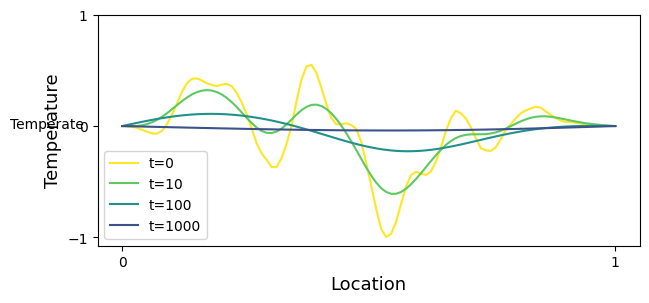
\includegraphics[width=1\columnwidth]{../images/1D_heat.png}
        \captionof{figure}{Numerical solution of the heat equation on $(0,1)\subset \reals$, with Dirichlet BCs $u(0, 0)=u(0, 1)=0$. The solution is shown at four curated timesteps. As time increases, the temperature distribution gets smoother, until it reaches $0$. Since the temperature moves towards the average, and the boundary is fixed at zero, the temperature must go to zero.}
        \label{fig:heat_1d}
    \end{center}
}
\subsection*{Method of Lines}
The challenge with ODEs was the continuous parameter $t$, which we overcame by discretizing across the temporal dimension. However, our PDEs now additionally depend on continuous spatial parameters $\mathbf{x}$. The Method of Lines (MOL) \cite{mol} works by converting the PDE to a system of ODEs, for which existing ODE solvers can be used. To convert to a system of ODEs, the only continuous parameter $u$ may depend on is $t$. By discretizing space into finite set of points $\mathbb{X} = (\mathbf{x}_1, \dots, \mathbf{x}_n)$, the continuous spatial input is been reduced to discrete indexing into $n$-vector $\mathbf{u}(t)$
$$\mathbf{u}(t) = \begin{bmatrix}
    u(t, \mathbf{x}_1), \dots, u(t, \mathbf{x}_n)
\end{bmatrix}^\top$$ 
containing the solution at each of the collocation points. However, having discretized space into a countable set of points, the differential operators acting on the spatial dimension are no longer defined. 
\definition{Finite Difference Methods}{
    Finite Differences (FD) methods approximate differential operators from regularly spaced finite points $\mathbb{X}$ of space. Standard differential operators are defined through limits, but with a finite number of spatial points, the limit must be approximated.
    This yields finite difference operators, which can be applied to a function evaluated at the same points $\mathbb{X}$ to approximate its spatial derivative in theses points.
    \\ 
    Like continuous differential operators, FD operators are only guaranteed to be defined on the interior of the domain. Supplying boundary conditions is therefore still necessary.
}
\definition{Collocation points}{
    In finite difference methods, collocation points are the spatial points where the finite difference approximations of derivatives are computed.
}
For linear differential operators the finite difference method will also be linear and can thus be written as a matrix. The exact form of the FD method depends on the discretization. In Euclidean space, rectangular grids yield simple formulas depending on the grid-spacing. On curved manifolds however, the grid-method breaks down. The methods from Discrete Exterior Calculus (ch. \ref{sec:manifolds}) give formulas for FD operators on discretized manifolds (triangle meshes). 
\example{$\reals$ Finite Differences, Gradient}{
    In one dimension, from a finite set of collocation points $$\mathbb{X} = (x_1<\dots<x_n) \subset (0, 1)$$ spaced $h$ apart, one can approximate the first derivative of $u: (0, 1) \to \reals$ on the interior $x_i$ with the central difference 
    \begin{align*}
        \frac{\partial}{\partial x}u(x_i) &\approx \frac{u(x_{i+1}) - u(x_{i-1})}{x_{i+1} - x_{i-1}}
        \\&= \frac{u(x_{i+1}) - u(x_{i-1})}{2h} 
    \end{align*}
    This formula breaks down for points $x_1$ and $x_n$ at the boundary, for which boundary conditions must be incorporated into the matrix. We will choose Dirichlet BC with zero boundary, which leads to the following matrix representation $D\in \reals^{n\times n}$ acting on the discretized function $\mathbf{u}$:
    $$D\mathbf{u} = \frac{1}{2h}
    \begin{bmatrix}
        0 & 0 & 0 & 0 & \dots & 0
        \\-1 & 0 & 1 & 0 & \dots & 0
        \\ 0 & -1 & 0 & 1 & \ddots & 0
        \\ \vdots & \ddots & \ddots & \ddots & \ddots & \vdots
        \\ 0 & \ddots & -1 & 0 & 1 & 0
        \\ 0 & \dots & 0 & -1 & 0 & 1
        \\ 0 & \dots & 0 & 0 & 0 & 0
    \end{bmatrix}\mathbf{u}$$ 
    The first and final empty rows encode the Dirichlet BC.
}
\example{$\reals$ Finite Differences, Laplacian}{
    To approximate the second derivative, we use the central difference twice. 
    $$\frac{\partial^2}{\partial x^2}u(x_i) \approx \frac{u(x_{i+1}) - 2 u(x_i) + u(x_{i-1})}{2h}$$ 
    This leads to matrix (with Dirichlet BCs = $0$)
    $$L\mathbf{u} = \frac{1}{h^2}
    \begin{bmatrix}
    0 & 0 & 0 & 0 & \cdots & 0 \\
    1 & -2 & 1 & 0 & \cdots & 0 \\
    0 & 1 & -2 & 1 & \cdots & 0 \\
    \vdots & \vdots & \vdots & \vdots & \ddots & \vdots \\
    0 & 0 & \cdots & 1 & -2 & 1 \\
    0 & 0 & \cdots & 0 & 0 & 0 \\
    \end{bmatrix}\mathbf{u}
    $$
    The first and final empty rows encode the Dirichlet BC.
}
The discrete differential operator encodes the spatial structure of the domain, and can be used to convert the PDE to a system of ODEs. Note that, \textit{once the differential operator is discretized, there is no reference to the underlying metric or topological structure. This information is encoded exclusively in the differential operator,} which means that the Method of Lines can be applied to any PDE on any domain, provided the differential operator can be discretized.
We will give a formula for the discrete gradient and Laplacian on a triangle mesh in chapter \ref{sec:manifolds}.
\example{Method of Lines applied to the Heat Equation}{
    The heat equation (\ref{eq:heat_equation}) makes use the linear differential operator $\Delta$, the Laplacian. By discretizing into spatial points $n = |\mathbb{X}|$ and deriving a suitable matrix $L\in\reals^{n\times n}$ estimating $\Delta$, we get the system of $n$ ODEs
    $$\hspace*{-3mm}i\!\in\!\{1,.., n\}\!: \hspace{2mm} \frac{d}{dt}u(t)_i = -L_i u(t)  \in \reals \hspace{14mm}$$
    where $L_i$ the $i$th row of $L$.
    We can write it more eloquently in vector-form by stacking all the spatial points to get
    \begin{align}\label{eq:space_stack}
        \frac{d}{dt}u(t) = -L u(t) \in \reals^n
    \end{align}
    \\
    The solution in figure \ref{fig:heat_1d} was obtained using this exact method, for $\mathbb{X} = \{0, \frac{1}{100}, \frac{2}{100}, \dots, \frac{99}{100}, 1\}$ and the FD Laplacian matrix from the previous box.
}
\example{Method of Lines applied to the Wave Equation}{
    The wave equation describes the evolution of the height of a wave $u(t, \mathbf{x})$ at a point $\mathbf{x}$ and time $t$.
    \begin{align}\label{eq:heat_equation}
        \frac{\partial^2}{\partial t^2}u = -\Delta u
    \end{align}
    Here, the vector field now prescribes the second-time derivative of $u$. We proceed with the Method of Lines:
    \\ Discretize space into $n = |\mathbb{X}|$ spatial points, compute matrix $L$ approximating $\Delta$. Similarly to the heat equation, we end up with the system of $n$ $2$nd order ODEs 
    $$\frac{d^2}{dt^2}u(t) = -L u(t) \in \reals^n$$
    As we prefer feeding $1$st order ODEs to our solvers, we will convert our $n$ second order ODEs to $2n$ first-order ODEs with the stacking equation (\ref{eq:stack})
    $$\frac{d}{dt}\vec{u} = \frac{d}{dt} \begin{pmatrix}
        u \\ v
    \end{pmatrix}= \begin{pmatrix}
        v \\ -L u
    \end{pmatrix}
    \in \reals^{2n}
    $$
    By linearity of $L$ we now apply the idea of eq. \ref{eq:linear_stack} to write everything as a single system matrix
    $$= \begin{bmatrix}
        \textbf{0} & \text{I}_n \\ -L & \textbf{0}
    \end{bmatrix} \begin{pmatrix}
        u \\ v
    \end{pmatrix} = A \vec{u_i}
    $$
    A is of dimension $2n \times 2n$ but highly sparse. The identity matrix $\text{I}_n$ plays the same role as the "$1$" in eq. \ref{eq:linear_stack}.
}
The sparse block-pattern in high derivative-order system matrices will be repeated in chapter \ref{sec:prior} where we will specify prior distributions over state-space encoded PDE solutions. For good measure, we will take a few more examples of linear PDEs and give their resulting system matrix.

\example{MOL on different PDEs and their 1st Order ODE Representation}{
    In the following table, $\textbf{I}$ is the $n\times n$ identity matrix, and $\mathbf{0}$ the $n\times n$ zero matrix.
        \hspace*{-2mm}\begin{tabular}{c|c|c}
        \hline 
        Linear PDE & System Mat. & $\vec{u}$
        \\\hline \hspace*{2mm} & \hspace*{2mm} 
        % START
        \\$\frac{\partial}{\partial t}u = -\Delta u$ & $\begin{bmatrix}
            -L
        \end{bmatrix}$ & $\begin{pmatrix}
            u
        \end{pmatrix}$
        \\ \hspace*{2mm} & \hspace*{2mm} 
        % END
        
        % START
        \\\hline \hspace*{2mm} & \hspace*{2mm} 
        \\$\frac{\partial^2}{\partial t^2}u = ku  -d\Delta \frac{\partial}{\partial t}u$ & $\begin{bmatrix}
            \textbf{0} & \textbf{I} \\ k\textbf{I} & -dL
        \end{bmatrix}$ & $\begin{pmatrix}
            u \\ v
        \end{pmatrix}$
        \\ \hspace*{2mm} & \hspace*{2mm} 
        % END
        
        % START
        \\\hline \hspace*{2mm} & \hspace*{2mm} 
        \\$\frac{\partial^2}{\partial t^2}u = a\Delta \frac{\partial}{\partial t}u$ & 
        $\begin{bmatrix}
            \textbf{0} & \textbf{I} 
            \\ \textbf{0} & aL
        \end{bmatrix}$ 
        & $\begin{pmatrix}
            u \\ v
        \end{pmatrix}$
        \\ \hspace*{2mm} & \hspace*{2mm} 
        % END

        % START
        \\\hline \hspace*{2mm} & \hspace*{2mm} 
        \\$\frac{\partial^3}{\partial t^3}u = \Delta u$ & 
        $\begin{bmatrix}
            \textbf{0} & \textbf{I} & \textbf{0}
            \\\textbf{0} & \textbf{0} & \textbf{I}
            \\ L & \textbf{0} & \textbf{0}
        \end{bmatrix}$ 
        & $\begin{pmatrix}
            u \\ v_1 \\ v_2
        \end{pmatrix}$
        \\ \hspace*{2mm} & \hspace*{2mm} 
        % END
        % START
        \\\hline \hspace*{2mm} & \hspace*{2mm} 
        \\$\frac{\partial^4}{\partial t^4}u = \Delta u + a\frac{\partial^2}{\partial t^2}u $ & 
        $\begin{bmatrix}
            \textbf{0} & \textbf{I} & \textbf{0} & \textbf{0}
            \\\textbf{0} & \textbf{0} & \textbf{I} & \textbf{0}
            \\ \textbf{0} & \textbf{0} & \textbf{0} & \textbf{I}
            \\ L & \textbf{0} & \!\!a\textbf{I} \!\!& \textbf{0}
        \end{bmatrix}$ \!
        & $\begin{pmatrix}
            u \\ v_1 \\ v_2 \\ v_3
        \end{pmatrix}$
        \\ \hspace*{2mm} & \hspace*{2mm} 
        % END
    \end{tabular}
    % TODO add label
    \\
    \\
    Notice the presence of the off-diagonal series of $\textbf{I}$. For an order $q$ PDE (or ODE), the upper $q\cdot n$ rows of the system Matrix will have this pattern to encode the derivatives.
}\noindent
Approximating the spatial derivatives is a simplified model, which is a source of error. The Probabilistic Numerical Solution in this thesis only models the error from time-discretization.
\example{Error Introduced by Spatial Discretization}{
    The Method of Lines proceeds in two independent steps, spatial discretization and temporal discretization. The way these two steps introduce approximation error are however \textit{not} independent. The error from a coarse spatial resolution can not be alleviated by arbitrarily increasing the temporal resolution and vice-versa. In \cite{pnmol} the authors propose the \textit{Probabilistic Numerical Method of Lines}, which quantifies the discretization error with probabilistic finite-difference methods. TODO Yes?
}

\ifdefined\COMPILINGFROMMAIN
\else    
    \end{document}
\fi